%\documentclass[letterpaper, 10 pt, conference]{orbieeeconfpre}
%\conference{IEEE Conference for Awesome ORB Research}
\documentclass[a4paper, 10pt, journal]{wissarbIEEE}

\bibliographystyle{orbref-num}
\IEEEoverridecommandlockouts	%  defines \thanks command 
\overrideIEEEmargins			% Needed to meet printer requirements.

\usepackage{hyperref}
\usepackage{graphicx}
\usepackage{tabularx}
\usepackage{booktabs}
\usepackage{cite}
\usepackage{xltabular}

\title{\LARGE \bf Neural Networks for Tool Image Classification}

\author{Boas Bamberger $^{1}$, Oliver Erlenkaemper$^{2}$ and Fabian Wolf$^{3}$ 
\thanks{$^{1}$Scientific Supervisor {\tt\small bamberger@uni-mannheim.de}} \thanks{$^{2}$Business Supervisor {\tt\small oliver.erlenkaemper@honeywell.com}} \thanks{$^{3}$Author {\tt\small s172298@student.dhbw-mannheim.de}}
}


\begin{document}
%acronyms
% Tool Image Classification Dataset (TIC Dataset)
\maketitle
\begin{abstract}
Augmented reality solutions for field workers are an emerging market.\cite{EY.2019a, EY.2019b, Detzel.2018, Shook.2019, Guy.2019} An augmented reality solution for field workers requires software perceiving the environment of field workers. A sub-task of that perception is the classification of different tools.
% Forschungsziel
We seek to determine the best-performing neural network for tool image classification.
% Methode
Furthermore, we introduce a novel dataset for tool image classification (TIC Dataset). To determine the best-performing neural network for tool image classification we train and evaluate neural networks on the TIC Dataset. We select the neural networks for the experiment based on a literature review which we conducted.
% Ergebniss
We found that, in general, not one particular but several neural networks are suitable for tool image classification, especially neural networks using convolutional layers and skip connections.
\end{abstract}

\section{Introduction}
\label{sec:intro}
Augmented reality solutions for field workers are an emerging market.\cite{EY.2019a, EY.2019b, Detzel.2018, Shook.2019, Guy.2019} An augmented reality solution for field workers requires software perceiving the environment of field workers. A sub-task of that perception is the classification of different tools. For example, a software displaying step-by-step instructions in the field of vision of a field worker needs to distinguish a screwdriver from a wrench when telling the field worker to tighten the screw with the wrench lying on the ground next to him instead of the screwdriver in his hand. This task is called tool image classification. We seek to determine the best-performing neural network for tool image classification. Furthermore, we introduce a novel dataset for tool image classification the TIC Dataset. To determine the best-performing neural network for tool image classification we train and evaluate neural networks on the TIC Dataset. We select the neural networks for the experiment based on a literature review which we conducted. Our time and resources were limited. For this reason, we exclusively train the neural networks supervised without auxiliaries. On that account, we exclude metalearning, especially neural architecture search, non-neural machine learning models, other computer vision tasks, unsupervised learning, semi-supervised learning, transfer learning, adversarial training, data augmentation, input normalization, weight decay, and multi-task learning. The following sections of this paper are structured as follows. Section \ref{sec:relwork} introduces related work and explains fundamentals required to understand this paper. Section \ref{sec:metho} defines the methodology followed to determine the best-performing neural network for tool image classification. Section \ref{sec:eval} reports the results of the experiment conducted by this paper. Section \ref{sec:discussion} discusses the results and reflects on the limitations of our work. Section~\ref{sec:conclusion} summarizes the contributions of this paper and proposes future work.
% TODO introdcuced dataset under CC SA
\section{Related Work}
\label{sec:relwork}
We seek to determine the best-performing neural network for tool image classification. To the best of our knowledge our paper is the first paper on tool image classification. Tool image classification is a subtask of image classification which is an advanced field and mostly solved by neural networks. Neural networks achieve accuracies of $96.08\%-98.66\%$\cite{Foret.2020, Kabir.2020} on , CIFAR \cite{cifar.2012}, MNIST \cite{mnist.2010}, SVHN \cite{svhn.2011}, STL\cite{stl.2011} and $88.61\%$\cite{Foret.2020} on ImageNet Dataset \cite{imagenet.2019} which comprises $1000$ classes and $3.2$ million images. Especially convolutional neural networks (CNNs) \cite{LeCun.2015b}, residual neural networks \cite{He.2016}, inception networks\cite{Szegedy.2015} and dense neural networks \cite{Huang.2017} have advanced the field.

\section{Method}
\label{sec:metho}
We determine the best-performing neural network for tool image classification in the course of an experiment on the TIC Dataset. Optimally, we would conduct a neural network architecture search and hyperparameter search for the experiment, but since our computational resources are limited we select the neural networks for the experiment based on a literature review which we conducted.

\subsection{Dataset Construction}
The TIC Dataset is a dataset for tool image classification. Thus, we created images consisting of exactly one tool of different classes. We chose the classes based on the tools which were freely available to us. The resulting classes are drill, hammer, pliers, saw, screwdriver and wrench.  In real world scenarios, tools are presented
from various angles and with various backgrounds. Due to this, the created images
are taken from arbitrarily chosen angles and with arbitrarily chosen backgrounds. We took all images of one class before taking images of another class and stored
them in different folders. The resulting folder structure is comprised by a root folder
containing one folder for each image class. Consequently the images are  inherently labeled by the folder structure. To  create an image we placed a tool in an arbitrarily chosen position and took a series of close-up images. During the series, the camera was moved around to create arbitrary angles. For the next series, the tool, the background,
and/or the position of the tool was changed.

\subsection{Model Selection}
We selected the neural networks based on a literature review. The literature review was conducted according to the method of\cite{Webster.2002} to examine the state of the art of image classification in regard to neural network architectures. For each architecture we selected one neural network for the experiment. Since the best-performing neural network on the ImageNet Dataset for each architecture uses more RAM than available to our limited hardware \cite{Foret.2020, Kolesnikov.2019, Touvron.2019}, we selected the neural network from the paper originally proposing the architecture.

\subsection{Experiment}
We split the TIC Dataset $60\%/20\%/20\%$ into training development and test dataset.
We train each neural network on the training dataset, tune its hyperparameters on the development dataset and evaluate it only once on the test dataset to prevent overfitting the test data. To conduct the experiment, we were provided $200$ hours on an Amazon Web Service g4dn.xlarge instance running a Deep Learning AMI (Ubuntu 18.04).\cite{AWS.2020a}
The g4dn.xlarge instance provides 4 vCPUs, 16GB RAM, 125GB storage, and a NVIDIA~T4~GPU. \cite{AWS.2020b} 
We implemented the experiment in Python 3\cite{Python3} using Keras~2.2.4.2\cite{Keras}, Tensorflow 2.1.0\cite{Tensorflow.2015}, CUDA 10.1\cite{CUDA}, and cuDNN 7.5.0\cite{cuDNN}.
\par
Training and hyperparameter tuning was executed exactly as in the paper originally proposing the neural network, except for dataaugmentation, weight decay and dropout which we excluded in this paper, see Section \ref{sec:intro}. Furthermore, we needed to adept the batchsize to the size of the available GPU RAM. We evaluated the performance of each neural network on the test dataset in accuracy.

\section{Evaluation}
\label{sec:eval}
The accuracy for each neural network on the TIC Dataset is reported in Table \ref{tab:acc}. For comparison we also report the original accuracy for each  neural network on the ImageNet Dataset.
Among these neural networks, DenseNet-264 performs best for the {TIC Dataset}. ResNet-152, ResNeXt-101, and DenseNet-264 perform rather similar. Therefore, we conclude that several neural networks are suited for tool image classification.  
EfficientNet-B7 achieved an accuracy of $16.67\%$ meaning it did not learn at all.
\begin{table}[h]
\caption{Experiment Results} \label{tab:acc}
	\begin{tabularx}{0.48\textwidth}{Xcc}
		\toprule 
		\textbf{Neural Network} & \textbf{TIC Dataset} & \textbf{ImageNet} \\\midrule
		VGG-19 & $72.40$ & $76.3$ \cite{Simonyan.2014}\\
		ResNet-152 & $92.89$ & $78.57$ \cite{He.2016}\\
		ResNeXt-101 & $94.66$ & $79.6$\cite{Xie.2017} \\
		\textbf{DenseNet-264} & $\mathbf{97.45}$ & $77.85$ \cite{Huang.2017}\\
		EfficientNet-B7 & $16.67$ & $84.4$ \cite{Tan.2019}\\
		\bottomrule
	\end{tabularx}
\end{table}

\section{Discussion}
\label{sec:discussion}
We found that, in general, several neural networks are suitable for tool image classification. This is in accordance with the state of the art of image classification, as image classification leaderboards show that different neural networks perform rather similarly for different image classification tasks. \cite{imagenet.2019, cifar.2012, mnist.2010, svhn.2011, stl.2011, clothing.2016, fashionMNIST.2017, Darlow.2018, flowers.2008, food.2014, vanHorn.2018, stanfordcars.2013, emnistletters.2017, kuzushijiMNIST.2018, cub.2011, Sabour.2017, isic1.2019, isic2.2018, isic3.2018}
\par
Especially, we found, that ResNet-152, ResNeXt-101, and DenseNet-264 are suitable for tool image classification. This also was to be expected since, ResNet-152, ResNeXt-101, and DenseNet-264 are suitable for image classification in general. \cite{Xie.2017, He.2016, Huang.2017} Despite differing in structure, each of these neural networks uses convolutional layers and skip connections. \cite{Xie.2017, He.2016, Huang.2017} This might be the cause of the similar performance. In comparison to these neural networks, VGG-19 performs less well. VGG-19 does not use skip connections. \cite{Simonyan.2014} Thus, we conclude, not using these connections might be the cause of the lower performance of VGG-19.
\par
In comparison to the ImageNet Dataset ResNet-152, ResNeXt-101, and DenseNet-264 perform better on the TIC Dataset, this might be due to the different complexity of the datasets. ImageNet Dataset has $1000$, while the TIC Dataset has $6$. Furtheremore the classes are completely different. Accordingly the complexity of classification is different for each class.
%TODO VGG schlechter => learning aux?
\par
EfficientNet-B7 did not learn at all. This might be, because, due to the limited GPU RAM, we were only able to train EfficientNet-B7 with a batch size of $1$. A batch size of $1$ causes the loss function to fluctuate heavily. This impairs convergence to the optimum and thus learning. On that account, the accuracy of EfficientNet-B7 reported in Section \ref{sec:eval} cannot be interpreted as the performance of EfficientNet-B7 for tool image classification, but simply as that EfficientNet-B7 was not able to learn in the course of the experiment.
We excluded metalearning, especially neural architecture search, non-neural machine learning models, other computer vision tasks, unsupervised learning, semi-supervised learning, transfer learning, adversarial training, data augmentation, input normalization, weight decay, and multi-task learning. On that account, it is likely, that even higher accuracies can be achieved using these techniques in addition to our approach.

\section{Conclusion}
\label{sec:conclusion}
We conclude that, for tool image classification convolutional neural networks using skip connections are suited. For industry aiming to create augmented reality solutions for field workers our implementation can be used as basic module of software perceiving the environment of field workers. 
For future work, we propose to improve our work with more performant hardware and additional training data to implement metalearning, semi-supervised learning, transfer learning, adversarial training, data augmentation, input normalization, weight decay, and multi-task learning, since these techniques were shown to improve performance. \cite{Pan.2010, Szegedy.2014, ElAmir.2020} 
Furthermore, we propose future work on the implementation of a holistic augmented reality solution for field workers, i.e. further computer vision tasks, a software framework, and a hardware framework for implementation.
\bibliography{bibliography}
\end{document}

%================================EXAMPLES================================
% use \CITE
% use \section and \subsection, don't use \chapter

% Figure
%\begin{figure}[h]
%   \centering
%   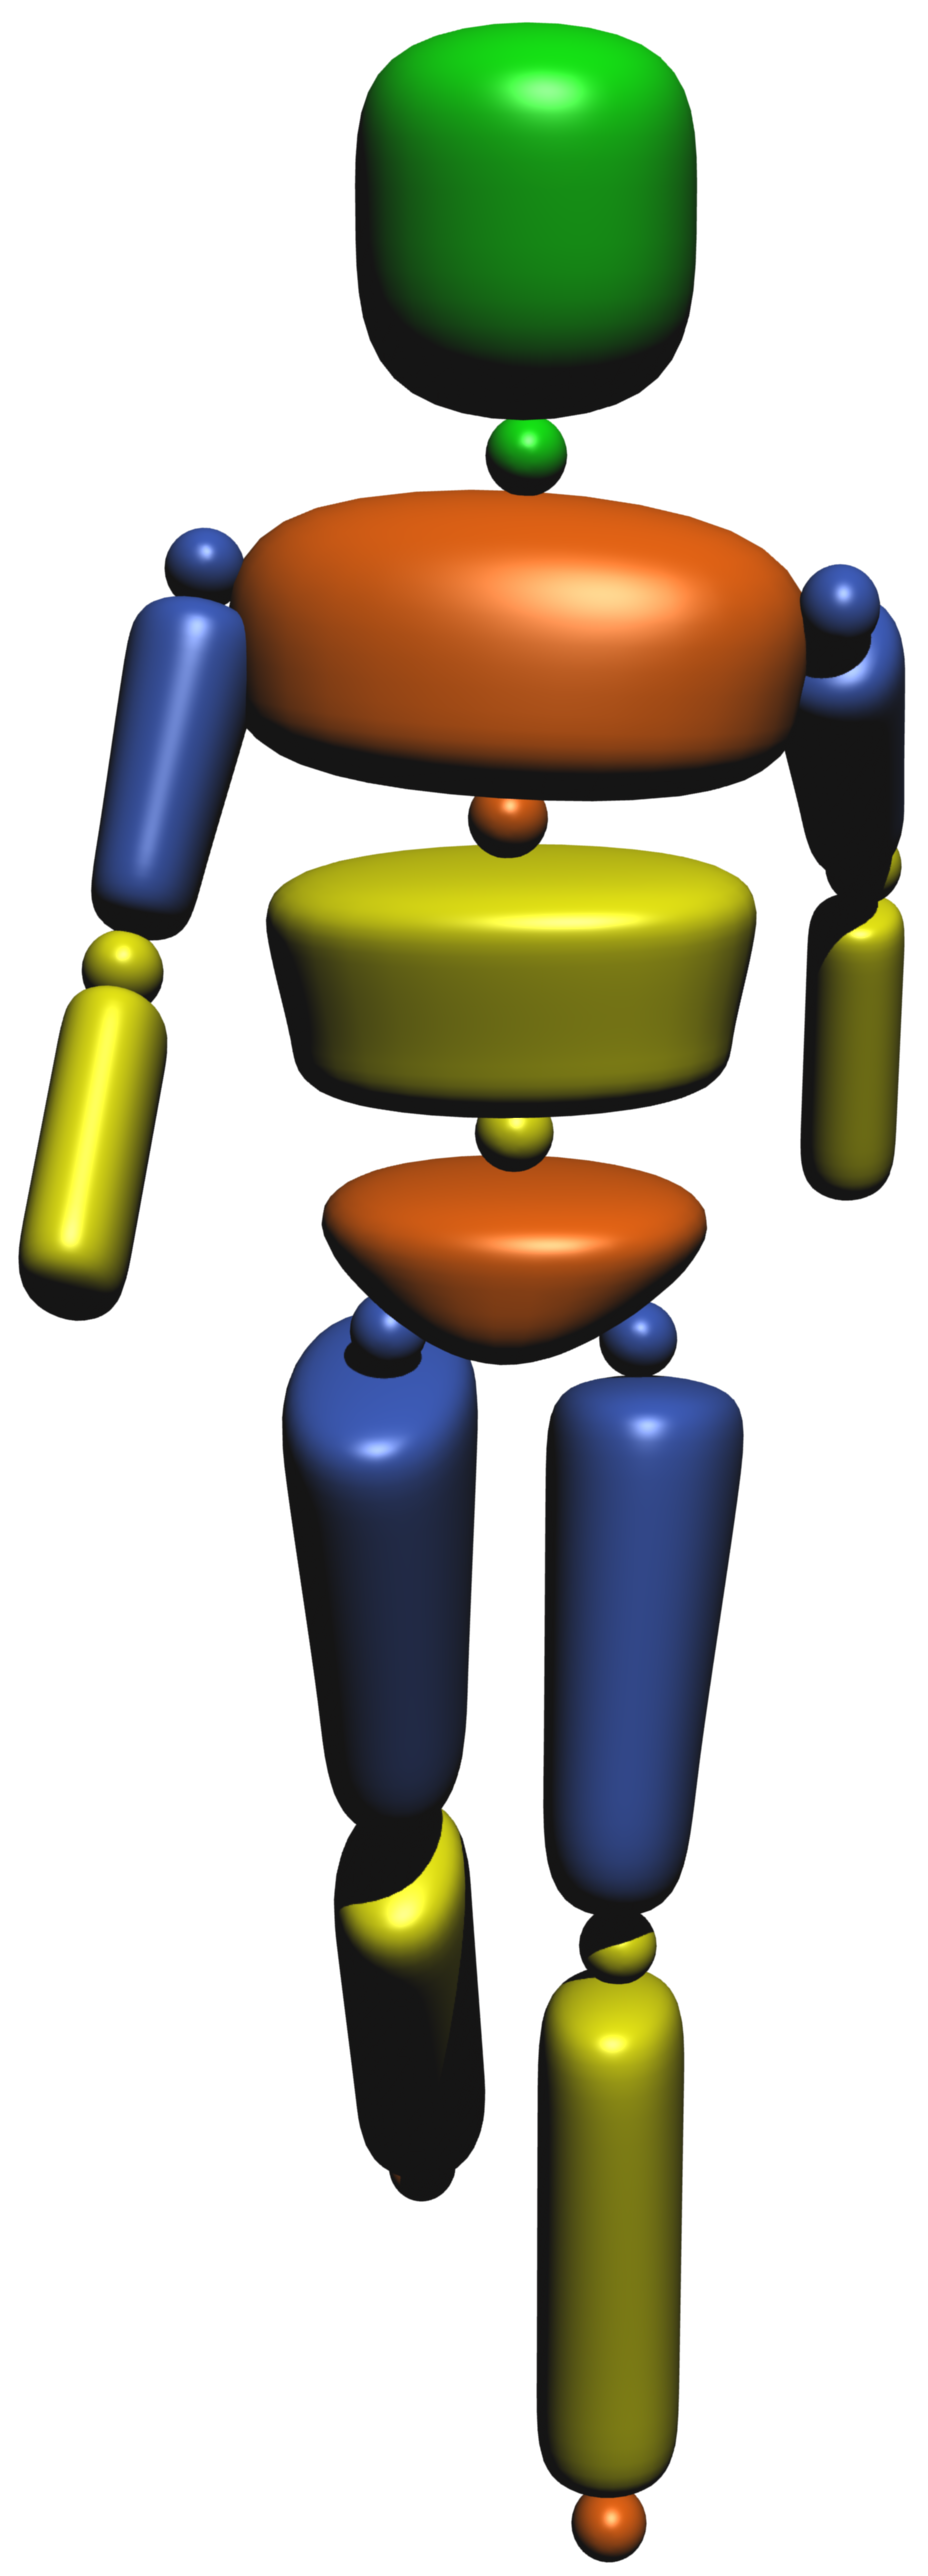
\includegraphics[width=0.1\textwidth]{fig/knubbi.png}
%   \caption{Example picture.}
%   \label{fig:knubbi}
%\end{figure}

% Table
%\begin{table}[h]
%\caption{Example table.}
%   \begin{tabularx}{0.48\textwidth}{llr}
%   		 \toprule 
%   		 Symbol & \multicolumn{1}{X}{Description} & Value [m] \\
%		 \midrule
%		  $A_x$ & Horizontal coordinate of A$^{*}$ & 0.0745 \\
%		  $A_z$ & Vertical coordinate of A$^{*}$ & 0.2650 \\  \noalign{\smallskip}
%		  
%		  $C_x$ & Horizontal coordinate of C$^{\#}$ & 0.0700 \\
%		  $C_z$ & Vertical coordinate of C$^{\#}$ & 0.1000 \\
%		  $D_x$ & Horizontal coordinate of D$^{\dag}$ & 0.0602 \\
%		  $D_z$ & Vertical coordinate of D$^{\dag}$ & 0.0860 \\
%		 \bottomrule
%   \end{tabularx}  \label{tab:initmodel}
%\end{table}